\subsection{Results for $y$ Offset}
%\label{subsec:latitude_no_abs_results}
%\vspace{10pt}

Figure~\ref{fig:var_lat} represents the $p$-values for the Wilcoxon signed-rank test on actual and predicted values across $k$-fold validation datasets for the $y$ offset in the $k$-fold testing datasets using different RNN models, and forecasting times. Darker colors in grayscale represent a higher $p$-value in a range from $0$ to $1$. The values on the secondary diagonal are all equal to $1$ and black because models equal themselves.

\begin{figure}[!ht]
	\centering
	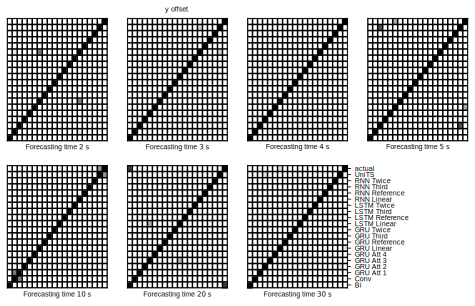
\includegraphics[width = 0.99 \linewidth]{var_lat.pdf}
	\caption{The $p$-values for the Wilcoxon signed-rank test on actual and predicted values across $k$-fold validation datasets for the $y$ offset in the $k$-fold testing datasets using different RNN models, and forecasting times. Darker colors in grayscale represent a higher $p$-value in a range from $0$ to $1$. The values on the secondary diagonal are all equal to $1$ and black because models equal themselves.}
	\label{fig:var_lat}
\end{figure}

The average $R^{2}$ (\%), with standard deviation in brackets, across $k$-fold validation datasets for the $y$ offset estimated on the $k$-fold testing datasets by different RNN models, and forecasting times is listed in Table~\ref{tab:best_latitude_no_abs_R2}.

\begin{table}[!ht]
	\centering
	\resizebox{\linewidth}{!}{
		\begin{tabular}{|c|c|c|c|c|c|c|c|}
			\hline
			Model & $2$ $s$ & $3$ $s$ & $4$ $s$ & $5$ $s$ & $10$ $s$ & $20$ $s$ & $30$ $s$ \\ \hline
			\multirow{2}{*}{Conv} & $93.52\%$ & $90.43\%$ & $86.78\%$ & $83.0\%$ & $64.03\%$ & $40.69\%$ & $\mathbf{29.8\%}$ \\
			 & ($1.09\%$) & ($1.02\%$) & ($1.17\%$) & ($1.44\%$) & ($2.07\%$) & ($2.47\%$) & \textbf{(}$\mathbf{1.4\%}$\textbf{)} \\ \hline
			\multirow{2}{*}{GRU Att 2} & $93.23\%$ & $90.0\%$ & $\mathbf{87.69\%}$ & $\mathbf{84.05\%}$ & $61.6\%$ & $28.71\%$ & $2.39\%$ \\
			 & ($1.51\%$) & ($2.05\%$) & \textbf{(}$\mathbf{1.72\%}$\textbf{)} & \textbf{(}$\mathbf{1.93\%}$\textbf{)} & ($3.4\%$) & ($6.2\%$) & ($8.4\%$) \\ \hline
			\multirow{2}{*}{GRU Reference} & $\mathbf{95.61\%}$ & $87.54\%$ & $80.31\%$ & $74.42\%$ & $45.82\%$ & $2.42\%$ & $-20.58\%$ \\
			 & \textbf{(}$\mathbf{2.14\%}$\textbf{)} & ($4.07\%$) & ($4.96\%$) & ($4.09\%$) & ($4.34\%$) & ($5.99\%$) & ($7.07\%$) \\ \hline
			\multirow{2}{*}{LSTM Third} & $93.81\%$ & $\mathbf{90.91\%}$ & $82.5\%$ & $77.25\%$ & $46.06\%$ & $1.72\%$ & $-20.76\%$ \\
			 & ($3.93\%$) & \textbf{(}$\mathbf{5.23\%}$\textbf{)} & ($8.75\%$) & ($5.43\%$) & ($3.94\%$) & ($5.94\%$) & ($9.82\%$) \\ \hline
			\multirow{2}{*}{UniTS} & $92.75\%$ & $89.96\%$ & $86.92\%$ & $83.77\%$ & $\mathbf{68.0\%}$ & $\mathbf{41.68\%}$ & $24.17\%$ \\
			 & ($1.98\%$) & ($1.67\%$) & ($1.63\%$) & ($1.67\%$) & \textbf{(}$\mathbf{2.31\%}$\textbf{)} & \textbf{(}$\mathbf{3.95\%}$\textbf{)} & ($4.68\%$) \\ \hline
		\end{tabular}
	}
	\caption{The average $R^{2}$ (\%), with standard deviation in brackets, across $k$-fold validation datasets for the $y$ offset estimated on the $k$-fold testing datasets by different RNN models, and forecasting times.}
	\label{tab:best_latitude_no_abs_R2}
\end{table}

The Conv model achieved the highest $R^{2}$ (\%) for $y$ offset, and a forecasting time of $30$ $s$ with an average value and standard deviation (in brackets) that equals $29.8$\% ($1.4$\%).

The GRU Att 2 model achieved the highest $R^{2}$ (\%) for $y$ offset, and a forecasting time of $4$, and $5$ $s$ with average values and standard deviation (in brackets) that equal $87.69$\% ($1.72$\%), and $84.05$\% ($1.93$\%) respectively.

The GRU Att 2 model does not make statistically significantly different predictions than the GRU Att 3 model for $y$ offset using a forecasting time of $4$ $s$, with a $p$-value equaling $2.656 \times 10^{-4}$.

\markertable{tab:\label{tab:latitude:no:abs:p:4}}

The GRU Reference model achieved the highest $R^{2}$ (\%) for $y$ offset, and a forecasting time of $2$ $s$ with an average value and standard deviation (in brackets) that equals $95.61$\% ($2.14$\%).

The LSTM Third model achieved the highest $R^{2}$ (\%) for $y$ offset, and a forecasting time of $3$ $s$ with an average value and standard deviation (in brackets) that equals $90.91$\% ($5.23$\%).

The LSTM Third model does not make statistically significantly different predictions than the LSTM Twice model for $y$ offset using a forecasting time of $3$ $s$, with a $p$-value equaling $6.104 \times 10^{-2}$.

\markertable{tab:\label{tab:latitude:no:abs:p:3}}

The UniTS model achieved the highest $R^{2}$ (\%) for $y$ offset, and a forecasting time of $10$, and $20$ $s$ with average values and standard deviation (in brackets) that equal $68.0$\% ($2.31$\%), and $41.68$\% ($3.95$\%) respectively.

The UniTS model does not make statistically significantly different predictions than the GRU Att 3, and actual value models for $y$ offset using a forecasting time of $10$ $s$, with $p$-values equaling $7.389 \times 10^{-3}$, and $4.075 \times 10^{-1}$.

\markertable{tab:\label{tab:latitude:no:abs:p:10}}

The UniTS model does not make statistically significantly different predictions than the actual value, and Bi models for $y$ offset using a forecasting time of $20$ $s$, with $p$-values equaling $6.866 \times 10^{-2}$, and $1.408 \times 10^{-3}$.

\markertable{tab:\label{tab:latitude:no:abs:p:20}}

The average MAE in $\degree$ ($\times 10^{-5}$), with standard deviation in brackets, across $k$-fold validation datasets for the $y$ offset estimated on the $k$-fold testing datasets by different RNN models, and forecasting times is listed in Table~\ref{tab:best_latitude_no_abs_MAE}.

\begin{table}[!ht]
	\centering
	\resizebox{\linewidth}{!}{
		\begin{tabular}{|c|c|c|c|c|c|c|c|}
			\hline
			Model & $2$ $s$ & $3$ $s$ & $4$ $s$ & $5$ $s$ & $10$ $s$ & $20$ $s$ & $30$ $s$ \\ \hline
			\multirow{2}{*}{GRU Att 1} & $\mathbf{5.558}$ & $\mathbf{7.454}$ & $8.885$ & $10.171$ & $20.701$ & $28.391$ & $32.677$ \\
			 & \textbf{(}$\mathbf{0.492}$\textbf{)} & \textbf{(}$\mathbf{0.708}$\textbf{)} & ($0.707$) & ($0.941$) & ($4.684$) & ($3.632$) & ($2.745$) \\ \hline
			\multirow{2}{*}{GRU Att 2} & $6.187$ & $7.917$ & $\mathbf{8.816}$ & $\mathbf{10.118}$ & $16.546$ & $23.948$ & $29.776$ \\
			 & ($0.608$) & ($1.082$) & \textbf{(}$\mathbf{0.762}$\textbf{)} & \textbf{(}$\mathbf{0.997}$\textbf{)} & ($1.513$) & ($2.1$) & ($2.891$) \\ \hline
			\multirow{2}{*}{GRU Att 4} & $5.863$ & $8.231$ & $9.942$ & $11.388$ & $\mathbf{16.223}$ & $26.774$ & $32.495$ \\
			 & ($0.526$) & ($0.708$) & ($0.854$) & ($1.044$) & \textbf{(}$\mathbf{1.953}$\textbf{)} & ($4.307$) & ($3.099$) \\ \hline
			\multirow{2}{*}{UniTS} & $7.176$ & $8.763$ & $10.181$ & $11.466$ & $16.562$ & $\mathbf{23.209}$ & $\mathbf{27.355}$ \\
			 & ($0.607$) & ($0.759$) & ($0.88$) & ($0.988$) & ($1.426$) & \textbf{(}$\mathbf{2.001}$\textbf{)} & \textbf{(}$\mathbf{2.3}$\textbf{)} \\ \hline
		\end{tabular}
	}
	\caption{The average MAE in $\degree$ ($\times 10^{-5}$), with standard deviation in brackets, across $k$-fold validation datasets for the $y$ offset estimated on the $k$-fold testing datasets by different RNN models, and forecasting times.}
	\label{tab:best_latitude_no_abs_MAE}
\end{table}

The GRU Att 1 model achieved the lowest MAE for $y$ offset, and a forecasting time of $2$, and $3$ $s$ with average values and standard deviation (in brackets) that equal $5.558 \times 10^{-5}$ $\degree$ ($0.492 \times 10^{-5}$ $\degree$), and $7.454 \times 10^{-5}$ $\degree$ ($0.708 \times 10^{-5}$ $\degree$) respectively.

The GRU Att 1 model does not make statistically significantly different predictions than the UniTS model for $y$ offset using a forecasting time of $2$ $s$, with a $p$-value equaling $1.373 \times 10^{-3}$.

\markertable{tab:\label{tab:latitude:no:abs:p:2}}

The GRU Att 2 model achieved the lowest MAE for $y$ offset, and a forecasting time of $4$, and $5$ $s$ with average values and standard deviation (in brackets) that equal $8.816 \times 10^{-5}$ $\degree$ ($0.762 \times 10^{-5}$ $\degree$), and $10.118 \times 10^{-5}$ $\degree$ ($0.997 \times 10^{-5}$ $\degree$) respectively.

The GRU Att 2 model does not make statistically significantly different predictions than the GRU Att 3 model for $y$ offset using a forecasting time of $4$ $s$, with a $p$-value equaling $2.656 \times 10^{-4}$.

The GRU Att 4 model achieved the lowest MAE for $y$ offset, and a forecasting time of $10$ $s$ with an average value and standard deviation (in brackets) that equals $16.223 \times 10^{-5}$ $\degree$ ($1.953 \times 10^{-5}$ $\degree$).

The GRU Att 4 model does not make statistically significantly different predictions than the LSTM Linear model for $y$ offset using a forecasting time of $10$ $s$, with a $p$-value equaling $1.121 \times 10^{-2}$.

The UniTS model achieved the lowest MAE for $y$ offset, and a forecasting time of $20$, and $30$ $s$ with average values and standard deviation (in brackets) that equal $23.209 \times 10^{-5}$ $\degree$ ($2.001 \times 10^{-5}$ $\degree$), and $27.355 \times 10^{-5}$ $\degree$ ($2.3 \times 10^{-5}$ $\degree$) respectively.

The UniTS model does not make statistically significantly different predictions than the actual value, and Bi models for $y$ offset using a forecasting time of $20$ $s$, with $p$-values equaling $6.866 \times 10^{-2}$, and $1.408 \times 10^{-3}$.

The UniTS model does not make statistically significantly different predictions than the GRU Att 2, GRU Linear, and actual value models for $y$ offset using a forecasting time of $30$ $s$, with $p$-values equaling $1.002 \times 10^{-1}$, $3.812 \times 10^{-3}$, and $1.084 \times 10^{-2}$.

\markertable{tab:\label{tab:latitude:no:abs:p:30}}

